\documentclass{article}
\usepackage{graphicx}
\usepackage[margin=1.5cm]{geometry}
\usepackage{amsmath}

\begin{document}

\title{Thursday Reading Assessment: Chapter 4}
\author{Prof. Jordan C. Hanson}

\maketitle

\section{Logic Circuits and Boolean Algebra}

\begin{enumerate}
\item (a) Write the boolean expression for the circuit in Fig. \ref{fig:gates1}.  (b) Convert the expression to S-SOP form, using $X+\bar{X} = 1$.  What is the domain number? \\ \vspace{2cm}
\begin{figure}[ht]
\centering
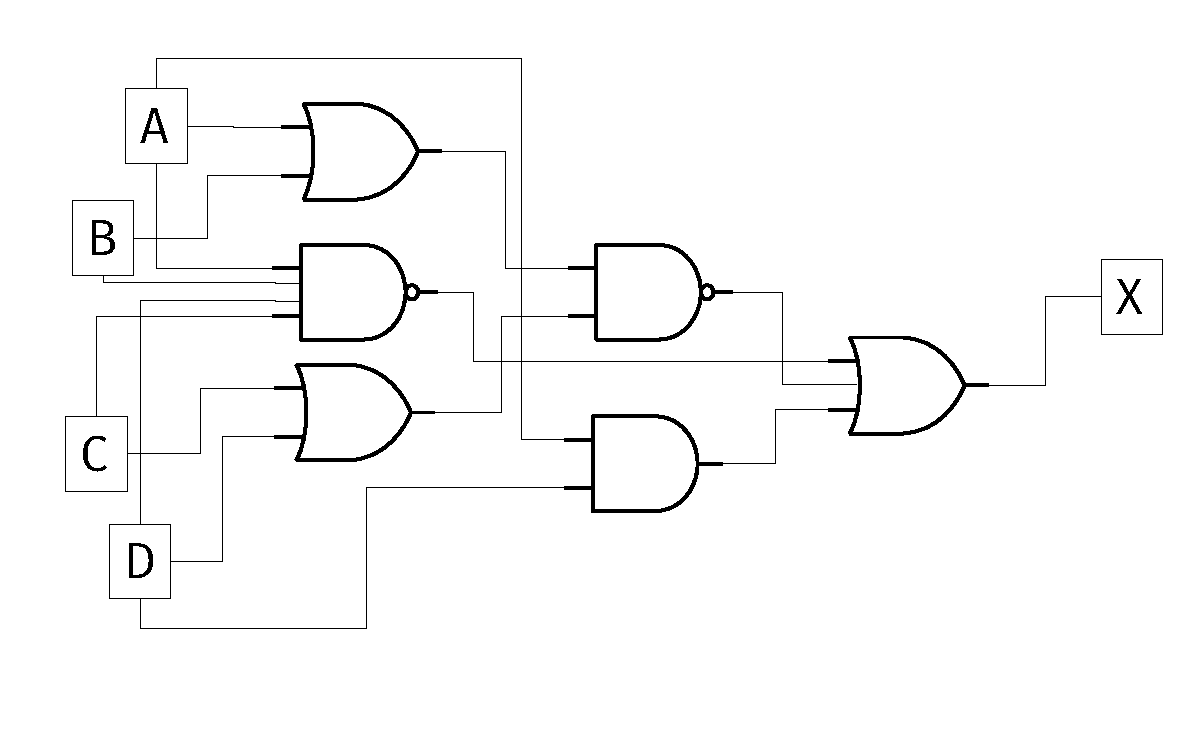
\includegraphics[width=0.5\textwidth]{figures/MultiGate1.pdf}
\caption{\label{fig:gates1} What is the logical expression for the output?}
\end{figure}
\item Determine the truth table (TT) for the circuit in Fig. \ref{fig:gates1}.
\end{enumerate}

\end{document}
